\chapter{Technische Unterschiede zwischen Xamarin.Forms und Flutter}
\label{chap:CrossPlattformFrameworks}

Die Unterschiede zwischen den Frameworks werden im folgenden genauer betrachtet.  Für den technischen Vergleich dient Xamarin.Forms als Grundlage.  Die Namen von Abschnitten und Unterabschnitten orientieren sich deshalb an dessen Terminologie.  In den jeweiligen Gliederungspunkten wird anschließend genauer betrachtet,  wie sich spezielle Arbeitsweisen oder Darstellungsoptionen in Flutter abbilden lassen. 

\section{Projektaufbau}
Xamarin.Forms weist eine andere Projektstruktur auf als Flutter,  das nur mit einem Projekt arbeitet.  Während das Flutter Projekt alle notwendigen Inhalte für iOS und Android inkludiert, \footcite[Vgl.][S. 113]{Biessek2019} setzt sich die sogenannte Lösung bei Xamarin.Forms aus mehreren Projekten zusammen.  Es gibt für jede Plattform ein dediziertes Projekt, das den plattformspezifischen Code,  Konfigurationen und Icons beinhaltet, sowie ein Projekt für den plattformunabhängigen Quelltext.   \footcite[Vgl.][S. 25f.]{Petzold2016} Icons und Konfigurationen werden bei Flutter in einem gleichen oder ähnlichen Format und nur in einem weiteren Projekt hinterlegt und lassen sich folglich migrieren.  


\subsection{Metadaten}
Zu den Metadaten einer Anwendungen gehören unter anderem der Name der Anwendung,  Informationen wie die benötigte Betriebssystemversion, das \glq App Launcher Icon\grq ,  das auf dem Smartphonebildschirm angezeigt wird und die Berechtigungen,  die von der mobile Anwendung während der Ausführung beantragt werden können.  Diese Eigenschaften werden bei Xamarin.Forms innerhalb der nativen Projekte verwaltet.  In iOS können Änderungen mittels der Datei \glq Info.plist\grq{} definiert werden. \footcite[Vgl.][Abgerufen am \today]{MicrosoftInfoPlist2017} Android speichert Metadaten innerhalb der \glq AndroidManifest.xml\grq{}. \footcite[Vgl.][Abgerufen am \today]{MicrosoftManifest2018} Flutter verwendet für die Verwaltung der Metadaten die identischen Dateien,  daher ist es möglich,  diese aus dem Xamarin.Forms Projekt zu kopieren und innerhalb des Flutter Projekts zu sichern.  Dafür muss die \glq Info.plist\grq im Verzeichnis \glq ios/Runner/\grq{} und die \glq AndroidManifest.xml\grq{}  in \glq android/app/src/main/\grq{} gespeichert werden.  In diesen Dateien wird außerdem der Identifizierer der Anwendung definiert.  Durch eine Kopie der Konfigurationsdatei und Erhöhung der Versionsnummer wird eine spätere Kompilierung der Flutter-App demnach als eine Aktualisierung der Xamarin.Forms App erkannt.  \footcite[Vgl.][Abgerufen am \today]{Rana2020}


\subsection{Bilder und Startbildschirm}
Innerhalb von Apps können Bilder das Benutzererlebnis verbessern und helfen,  eine Aktion zu veranschaulichen oder komplexe Botschaften zu verdeutlichen.  \footcite[Vgl.][Abgerufen am \today]{GoogleMaterialImages2020} In iOS und Android werden sie in verschiedenen Auflösungen bereit gestellt.  Das Betriebssystem wählt während der Laufzeit die beste Ressource basierend auf den Eigenschaften des Smartphonedisplays aus.  Xamarin.Forms verwendet die  \acfp{api} (auf deutsch Programmierschnittstellen) der nativen Plattformen zum Laden lokaler Bilder und unterstützt daher die plattformspezifischen Funktionalitäten.\footcite[Vgl.][Abgerufen am \today]{MicrosoftXamImages2020} Zur Verwendung nativer Bilddateien müssen die Bilder in Xamarin.Forms zu jedem Anwendungsprojekt hinzugefügt werden und vom gemeinsamen Xamarin.Forms-Code referenziert werden.  Flutter benutzt im Gegensatz zu Xamarin.Forms keine nativen \acp{api},  sondern ein einfaches Dichte-basiertes Format,  ähnlich dem von iOS.  Für die Anzeige von Bildern arbeitet Flutter mit sogenannten logischen Pixeln.  Alle Bilderressourcen können sich in einem beliebigen Ordner innerhalb des Projekts befinden, da Flutter keine vordefinierte Ordnerstrukturen hat. \footcite[Vgl.][Abgerufen am \today]{GoogleFlutterImages2020} Der Startbildschirm (engl. Splashscreen) ist der Einstiegspunkt der mobilen App unddient als Ladebildschrim.  Er wird bei Xamarin.Forms in den plattformspezifischen Projekten gespeichert und kann nicht wie die \glq Info.plist\grq - und die \glq AndroidManifest.xml\grq{}-Dateien in das Flutter Projekt kopiert werden,  da er in Android mithilfe von plattformspezifischem Quelltext implementiert ist. \footcite[Vgl.][Abgerufen am \today]{GoogleSplash2020} 


\subsection{Benutzerdefinierte Schriftarten}
Eine Schriftart (engl. Font) wird verwendet,  um das Design und den Inhalt so klar und effizient wie möglich darzustellen,  dafür haben Android und iOS  eine Vielzahl an Fonts vorinstalliert.  Wenn eine mobile App jedoch auf eine benutzerdefinierte Schriftart zurückgreifen möchte,  muss diese mit der Anwendung mitgeliefert werden.  In Xamarin.Forms mussten Fonts bis zum Jahre 2020 in jedem nativen Projekt referenziert werden.  Seit der Version 4.5 können diese Dateien auch plattformübergreifend verwendet werden und befinden sich daher innerhalb des geteilten Projekts. \footcite[Vgl.][Abgerufen am \today]{Versluis2020}  In Flutter werden die Fonts wie in der neueren Version von Xamarin.Forms in einem Ordner abgelegt. \footcite[Vgl.][Abgerufen am \today]{GoogleFlutterFonts2020}  Eine Verwendung des Schriftsatzes \glq MyCustomFont\grq{} in Flutter wird in Quelltext \ref{lst:FlutterFont} dargestellt.  

\lstinputlisting[label={lst:FlutterFont},caption={[Verwendung eines benutzerdefinierten Schriftsatzes in Flutter]{Verwendung eines benutzerdefinierten Schriftsatzes in Flutter\footcite[In Anlehnung an][Abgerufen am \today]{GoogleFlutterPackages2020}}}, language=Dart]{SourceCode/Fonts.Dart} 

\subsection{Plattformspezifischer Quelltext}
In\footcitetext[Quelltext in Anlehnung an][Abgerufen am \today]{GoogleFlutterFonts2020} den Ausschlusskriterien des dritten Kapitels wurde der plattformspezifische Quelltext von Xamarin.Forms für die Übersetzung exkludiert.  Der Vollständigkeit halber sollen die Unterschiede zwischen den Plattformen jedoch trotzdem erwähnt werden.  Xamarin.Forms unterteilt nativen Quelltext in zwei Kategorien, die sogenannten \glq DependencyServices\grq{} die es erlauben,  Funktionenalitäten in den Plattformprojekten aus dem geteilten Code aufzurufen, \footcite[Vgl.][Abgerufen am \today]{MicrosoftDependencyService2017}  sowie \glq Custom Renderers\grq,  die es ermöglichen das Aussehen und Verhalten von Steuerlementen anzupassen. \footcite[Vgl.][Abgerufen am \today]{MicrosoftCustomRenderers2017} In Flutter wird für die Ausführung von plattformspezifischen Funktionalitäten auf \glq platform-channels\grq{} zurückgegriffen. \footcite[Vgl.][Abgerufen am \today]{GooglePlatformspecificCode2020} Für \glq Custom Renderer\grq{}  gibt es bei keine Alternative, da das Framework keine nativen Steuerelemente verwendet,  sondern Widgets anzeigt. 

\section{Erweiterungen}
Erweiterungen sind Programmergänzungen, die auch von externen Entwicklern beigetragen werden können.  Sie dienen der Reduzierung des Entwicklungsaufwandes, da nicht jede Funktionalität eigens implementiert werden muss.  Im .NET-Ökosystem können Xamarin.Forms-Projekte auf das Paketverwaltungssystem Nuget zugreifen,  um Erweiterungen zu einer App hinzuzufügen. \footcite[Vgl.][Abgerufen am \today]{MicrosoftXamNuget2020}  Bei Flutter wird für diesen Fall mit der pubspec.yaml Datei eine Referenz auf das ausgewählte Plugin gesetzt.  Dabei werden in Dart geschriebene Pakete von plattformunabhängigen Plugins unterschieden.  Diese Plugins können für Android (mit Kotlin oder Java) oder für iOS (mit Swift oder Objective-C) geschrieben sein. \footcite[Vgl.][Abgerufen am \today]{GoogleFlutterPackages2020} In Quelltext \ref{lst:Pubspecjaml} wird ein Auschnitt der pubspec.yaml Datei gezeigt, in welcher das in Unterabschnitt \ref{sec:nav} erwähnte Plugin \glq url\_launcher\grq{}   geladen wird.

%Kein Quelltext- ggf ändern.
\lstinputlisting[label={lst:Pubspecjaml},caption={[Erweiterungen in Flutter]{Erweiterungen in Flutter\footcite[In Anlehnung an][Abgerufen am \today]{GoogleFlutterPackages2020}}}, language=Dart]{SourceCode/Pubspec.yaml} 
\footcitetext[Quelltext in Anlehnung an][Abgerufen am \today]{GoogleFlutterPackages2020}In dem Beispiel muss das Plugin mindestens die Version 5.4 haben,  darf jedoch die Version 6 nicht überschreiten.  Aufgrund der Vielzahl an existierenden Erweiterungen für beide Frameworks ist es nicht möglich,  eine vollständige Gegenüberstellung anzulegen.  Im Folgenden wird jedoch anhand von drei gängigen Anwendungsszenarien der Einsatz von Erweiterungen erläutert.

\subsection{Interaktion mit der Hardware}
Android und iOS nutzen einzigartige Betriebssystem- und Plattform-\acp{api},  auf die Xamarin.Forms Entwickler zugreifen können.  Mit der Erweiterung Xamarin.Essentials bietet Microsoft eine plattformübergreifende \ac{api}, auf die von gemeinsamem Code aus zugegriffen und die direkt auf der Plattform ausgeführt werden kann.  Der Dart Quelltext,  aus dem eine Flutter-App besteht, wird nicht auf der zugrundeliegenden Plattform, sondern nativ auf dem Gerät ausgeführt.  Es werden also nicht die iOS oder Android \acp{api} benutzt.  Flutter Apps können über Plattformkanäle jedoch auch mit den nativen \acp{api} interagieren,  um beispielsweise Daten von Sensoren des Gerätes abzurufen.\footcite[Vgl.][Abgerufen am \today]{GooglePlatformspecificCode2020}

\subsection{Speicherung von Daten}
Ein wesentlicher Bestandteil jeder mobilen Anwendung ist die Fähigkeit Daten zu persistieren.  Manchmal handelt es sich dabei um große Datenmengen,  die eine Datenbank erfordern,  oft sind es aber auch kleinere Daten, wie Einstellungen und Präferenzen, die zwischen den Starts der Anwendung gespeichert werden müssen.  

Für die Speicherung in einer Datenbank können Xamarin.Forms Entwickler auf verschiedene Lösungsansätze zurückgreifen.  Zum einen \glq SQLite\grq{}, die am häufigsten verwendete Datenbank-Engine der Welt\footcite[Vgl.][Abgerufen am \today]{SQLiteConsortium2020},  oder \glq Realm\grq{},  eine Datenbank optimiert für mobile Endgeräte. \footcite[Vgl.][Abgerufen am \today]{MongoDBRealm2020} Beide Datenbanken stehen auch als Plugin für \glq Flutter\grq{} zur Verfügung, wobei SQLite ausgereift ist,\footcite[Vgl.][Abgerufen am \today]{Tekartik2020} während \glq Realm\grq{} erst am 5 November 2020 Support für Flutter angekündigt hat und noch nicht offiziell zur Verfügung steht. \footcite[Vgl.][Abgerufen am \today]{MongoDBFlutterSupport2020}

Die Xamarin.Essentials Erweiterung stellt Entwicklern das \glq Settingsplugin\grq{} bereit, welches die Sicherung von Präferenzen und App-Einstellungen erlaubt.  \footcite[Vgl.][Abgerufen am \today]{MicrosoftXamSettings2019} In Flutter wird für diese Speicherung mit Hilfe des Plugins \glq shared\_preferences\grq{}  auf die gleichen plattformspezifischen \ac{api} zugegriffen.  \footcite[Vgl.][Abgerufen am \today]{GoogleFlutterSharedPreferences2020}  Die Verwendung der gleichen \acp{api} ist ein wichtiger Faktor, da die von Anwendern gespeicherten Daten  auch nach einem Frameworkwechsel zu Flutter noch verfügbar sind. 

\subsection{Navigation zu anderen Anwendungen}
\label{sec:nav}

Mobile Anwendungen können die Möglichkeit zur Navigation zu anderen Apps realisieren.  Dafür greift Xamarin Forms auf ein bestimmtes \ac{uri}-Schema zurück, mit dem Ressourcen eindeutig bezeichnet werden.  Durch den Befehl \glq Launcher.OpenAsync("mailto://")\grq{}, der Bestandteil der Xamarin.Essentials Erweiterung ist,  wird z.B.  das Standardprogramm für E-Mails des Smartphones gestartet. \footcite[Vgl.][Abgerufen am \today]{MicrosoftLauncher2020}  Mithilfe des Plugins \glq url\_launcher\grq{} kann die Funktionalität zum Öffnen von anderen Anwendungen zu Flutter Apps hinzugefügt werden.\footcite[Vgl.][Abgerufen am \today]{Googleurllauncher2020} Die unterstützten \ac{uri}-Schemata und ihre Aktionen werden in Tabelle \ref{tab:URISChema} dargestellt.

\begin{table}[!ht]
\begin{tabularx}{\textwidth}{|l|X|}
\hline
   \textbf{\ac{uri}-Schemata} & \textbf{Aktion}  \\
\hline
	http:<URL>		       				&  	URL wird im Standardbrowser geöffnet 		\\ 
	mailto:<E-Mail Adresse>		     		&  	Erstellt eine Email an die angegebene E-Mail Adresse 		\\ 
	tel:<Telefonnummer>	       		&  	Ruft die Rufnummer an 		\\ 
	sms:<Telefonnummer>		       		&  	Schreibt eine SMS an die Rufnummer		\\ 
	\hline
\end{tabularx}
\caption{Unterstützte Schemata des \glq url\_launcher\grq{} Plugins}
 \label{tab:URISChema}
\end{table}

\section{Lebenszyklus}
Durch das Navigieren zu anderen Anwendungen ändert sich der Status von Ausführung im Vordergrund zu Ausführung im Hintergrund.  Der aktuelle Status der App bestimmt die Handlungsoptionen.  Befindet sich eine App im Vordergrund, hat sie die Aufmerksamkeit des Benutzers und ist damit priorisiert beim Zugriff auf die Systemressourcen einschließlich der CPU.  Gleichzeitig muss eine Hintergrund-App möglichst inaktiv sein,  da sie sich außerhalb des Bildschirms befindet.  Mobile Anwendungen müssen auf Änderungen des Lebenszyklus-Status reagieren können, um ihr Verhalten entsprechend anzupassen.\footcite[Vgl.][Abgerufen am \today]{AppleLifecycycle2020} Xamarin.Forms bietet dafür die  drei Methoden \glq OnStart\grq{} , \glq OnResume\grq{} und \glq OnSleep\grq{} an,  die aufgerufen werden, wenn sich der Status verändert. \footcite[Vgl.][Abgerufen am \today]{MicrosoftXamLifecycle2020} Bei Flutter kann auf die \glq didChangeAppLifecycleState\grq{} Methode zurückgegriffen werden, die bei Änderungsereignissen ausgelöst wird und die ebenfalls die drei Lebenszyklen beinhaltet. \footcite[Vgl.][Abgerufen am \today]{GoogleFlutterLifeCycle2020} 

\section{Ansichten}
Ansichten (engl. Views) sind visuelle Elemente, die in zwei Kategorien unterschieden werden können.  Steuerelemente (engl. Controls) sind für die Sammlung von Benutzereingaben oder die Ausgabe von Daten zuständig,  Layouts beinhalten eine Sammlung von Ansichten und sind für ihre visuelle Anordung auf der Benutzeroberfläche verantwortlich.  \footcite[Vgl.][Abgerufen am \today]{Ritscher2020} Im folgenden Abschnitt werden Xamarin.Forms- und Flutter-Ansichten gegenübergestellt.  Damit soll ein Konzept für die Übersetzung von grafischen Benutzeroberflächen dargelegt und die Möglichkeiten des Austausches von Ansichten für den Compiler validiert werden.

\subsection{Layouts}
Ähnlich wie die Ansichten lassen sich auch die Layouts in zwei Kategorien unterteilen, Ansichtsseiten (engl. Pages) sowie die generellen Layouts.  Die Pages nehmen den gesamten Bildschirm ein und werden in Abbildung \ref{fig:Xamarin.Forms Pages} dargestellt.\footcite[Vgl.][Abgerufen am \today]{MicrosoftXamPages2016}  

\begin{figure}[!ht]
 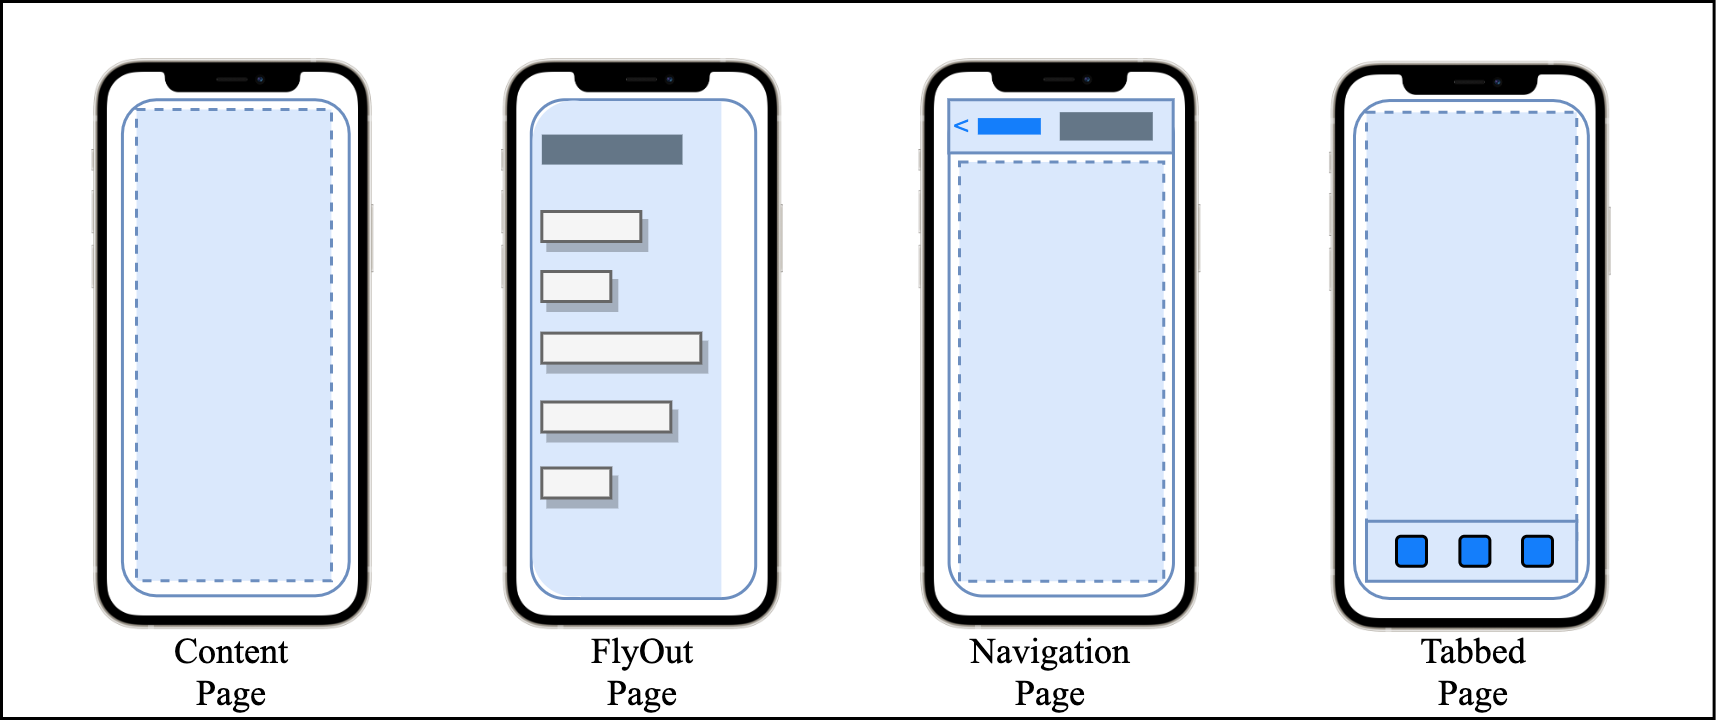
\includegraphics[width=\textwidth,height=\textheight,keepaspectratio]{Images/CrossPlattformFrameworks/XamarinFormsPages.png}
 \caption[Xamarin.Forms Pages]{Xamarin.Forms Pages\footcite{MicrosoftXamPages2016}}
 \label{fig:Xamarin.Forms Pages}
\end{figure}

Die \glq ContentPage\grq{} ist ausschließlich für die Anzeige einer weiteren Ansicht verantwortlich.  Die drei anderen Pages besitzen ein Navigationskonzept.  \footcitetext[Abbildung in Anlehnung an][Abgerufen am \today]{MicrosoftXamPages2016} Die \glq FlyOutPage\grq{} teilt den Bildschirm in zwei Bereiche, ein Bereich dient der Navigation.  Er enthält ein Menü das, wie im Namen enthalten, einfliegen kann.  Der zweite Bereich zeigt eine Detailansicht,  in welcher der Inhalt der angeforderten Seite geladen wird.  \glq NavigationPage\grq{} bietet eine Navigationsleiste, die einen Titel der aktuellen Seite und eine Navigationsschaltfläche beinhalten kann.  \glq TabbedPage\grq{} stellt die unterschiedlichen Seiten als Registerkarten dar. \footcite[Vgl.][Abgerufen am \today]{MicrosoftXamPages2016}
Die Ansichtsseiten befinden sich in der Regel innerhalb der \ac{xaml}-Datei auf der untersten Ebene, dem so genannten Wurzelknoten. Der Quelltext \ref{lst:TabbedPage} zeigt dies exemplarisch für eine \glq TabbedPage\grq{}.  

\lstinputlisting[label={lst:TabbedPage},caption={[Xamarin.Forms \glq TabbedPage\grq{} Definition]{Xamarin.Forms \glq TabbedPage\grq{} Definition\footcite[Quelltext in Anlehnung an][Abgerufen am \today]{MicrosoftXamTabbedView2020}}} , language=XML]{SourceCode/XamarinFormsTabbedPage.XAML}

\footcitetext[Quelltext in Anlehnung an][Abgerufen am \today]{MicrosoftXamTabbedView2020}Es wird eine \glq TabbedPage\grq{} mit zwei Registerkarten entworfen.  Eine Kombination mehrerer Navigationskonzepte ist  möglich,  das Beispiel zeigt eine Navigationsleiste innerhalb der Registerkarten. 

Die verfügbaren Eigenschaften der Ansichtsseiten unterscheiden sich je nach Einsatzszenario.  Im folgenden Quelltext \ref{lst:FlyOutPage} wird dies exemplarisch an der Realisierung einer \glq FlyoutPage\grq{} deutlich.  Anders als bei der \glq TabbedPage\grq{}, die aus einer Sammlung von Registerkarten besteht, finden sich im Quelltext die Eigenschaften \glq Flyout\grq{}  und \glq Detail\grq{}.

\lstinputlisting[label={lst:FlyOutPage}, caption={[Xamarin.Foerms \glq FlyoutPage\grq{} Definition]{Xamarin.Forms \glq FlyoutPage\grq{} Definition\footcite[Quelltext in Anlehnung an][Abgerufen am \today]{MicrosoftXamFlyOutPage2020}}} ,language=XML]{SourceCode/XamarinFormsFlyoutPage.XAML}

Im Gegensatz zu Xamarin.Forms kann Flutter auf der Wurzelebene nur den Style der App, \footcitetext[Quelltext in Anlehnung an][Abgerufen am \today]{MicrosoftXamFlyOutPage2020}
 nicht aber ein Navigationskonzept definieren.  Wie bereits in Kapitel \ref{chap:CompilerEntwurf} aufgeführt, wird in dieser Arbeit ausschließlich der Material Design Style unterstützt. \footcite[Vgl.][Abgerufen am \today]{FlutterForXFDevs} Quelltext \ref{lst:MaterialApp} zeigt die Realisierung einer \glq Material Design \grq{} App in Flutter.

\lstinputlisting[label={lst:MaterialApp}, caption={[Flutter \glq MaterialApp\grq{} Definition]{Flutter \glq MaterialApp\grq{} Definition\footcite[Quelltext in Anlehnung an][Abgerufen am \today]{GoogleFlutterFirstApp2020}}}, language=Dart]{SourceCode/MaterialApp.Dart}

Der Vergleich zwischen den XML basierten \ac{xaml}-Dateien\footcitetext[Quelltext in Anlehnung an][Abgerufen am \today]{GoogleFlutterFirstApp2020} und den bei Flutter verwendeten Dart-Dateien verdeutlicht die Unterschiede in den verwendeten Sprachen zur Benutzeroberflächenentwicklung.  Die zentrale Idee hinter dem Flutter-Framework ist es,  eine Benutzeroberfläche aus Widgets aufzubauen.  Diese beschreiben das Aussehen der Anwendung basierend auf ihrem aktuellen Zustand.  Sobald sich der Status ändert, kann das Framework den neuen mit dem alten Status vergleichen und grafische Veränderungen  effektiv vornehmen. \footcite[Vgl.][Abgerufen am \today]{GoogleWidgets2020} Um in Flutter ein Navigationskonzept zu definieren,  können verschiedene Widgets verwendet und verschachtelt werden,  wie in Quelltext \ref{lst:FlutterTabbedApp} beispielhaft für eine App mit Registerkarten visualisiert wird.

\lstinputlisting[label={lst:FlutterTabbedApp},caption={[Flutter \glq Tab Layout\grq{} Definition]{Flutter \glq Tab Layout\grq{} Definition\protect\footcite[Quelltext in Anlehnung an][Abgerufen am \today]{GoogleFlutterTabs2020}}}, language=Dart]{SourceCode/TabbedPage.Dart}
Die\footcitetext[Quelltext in Anlehnung an][Abgerufen am \today]{GoogleFlutterTabs2020}  deutlichen Unterschiede bei der Auswahl eines Navigationkonzeptes können überbrückt werden,  indem zu jeder Xamarin.Forms Page das entsprechende Flutter Widget gefunden wird.  Der Flutter-Widgetkatalog\footcite[Vgl.][Abgerufen am \today]{GoogleFlutterWidgetCatalog2020} und die Webseite "Flutter for Xamarin.Forms Developers"\footcite[Vgl.][Abgerufen am \today]{FlutterForXFDevs} wurde für die Recherche der Gegenstücke verwendet.  Entsprechende Ergebnisse der Suche können in Tabelle \ref{tab:ComparePAGESFlutter} abgelesen werden. 

\begin{table}[!ht]
\begin{tabularx}{\textwidth}{|X|X|}
\hline
   \textbf{Xamarin.Forms Page} & \textbf{Flutter Widget}  \\
\hline
	ContentPage            &           	\\ 
	FlyOutPage             & MasterDetailScaffold          	\\ 
	NavigationPage       & Scaffold         	 					\\ 
	TabbedPage            & TabBar und TabBarView 		\\ 
	\hline

\end{tabularx}
\caption{Gegenüberstellung von Pages}
 \label{tab:ComparePAGESFlutter}
\end{table}

Gegenüberstellungen von Xamarin.Forms Elementen und Flutter Widgets in Tabellenform werden auch an anderer Stelle in diesem Kapitel zugunsten der Übersichtlichkeit verwendet.  Flutter Widgets, die im Text nicht expliziert aufgeführt werden,  sind den Xamarin.Forms Elementen in Funktionalität und Aussehen nahezu identisch.  Eine vollständige Referenztabelle,  die sich aus allen Einzelbetrachtungen zusammensetzt,  befindet sich in \hyperref[chap:Gegenueberstellung]{Anhang I} .

Die Navigation durch die Anwendung ist ein wichtiger Bestandteil und hängt wie beschrieben von der verwendeten Ansichtsseite ab.  Die \glq NavigationPage\grq{} bietet eine hierarchische Navigation, bei der der Benutzer durch die Seiten vorwärts und rückwärts navigieren kann. \footcite[Vgl.][Abgerufen am \today]{MicrosoftXamNavigation2020} Flutter hat eine ähnliche Implementierung,  welche die Widgets  \glq  Navigator\grq{} und \glq  Routen\grq{} verwendet.  \footcite[Vgl.][Abgerufen am \today]{GoogleFlutterNavigation2020} 

Neben den Ansichtsseiten bietet Xamarin.Forms weitere Layouts,  die Steuerelemente zu visuellen Strukturen zusammenstellen.  Abbildung \ref{fig:Xamarin.Forms Layouts} präsentiert die gebräuchlichsten dieser Layouts. 

\begin{figure}[!ht]
 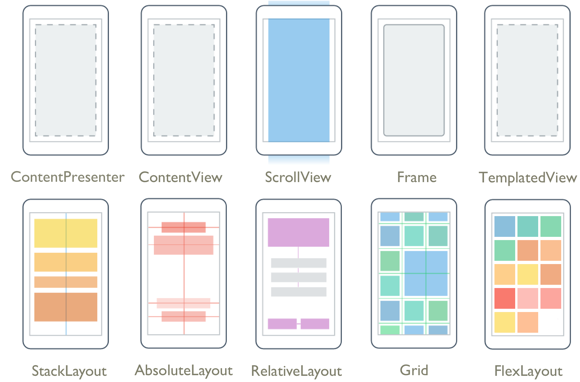
\includegraphics[width=\textwidth,height=\textheight,keepaspectratio]{Images/CrossPlattformFrameworks/XamarinFormsLayouts.png}
 \caption[Xamarin.Forms Layouts]{Xamarin.Forms Layouts\footcite{MicrosoftXamViews2020}}
 \label{fig:Xamarin.Forms Layouts}
\end{figure}

Die vorgestellten Layouts haben  unterschiedliche visuellen Eigenschaften und dienen als Sprachelemente von \ac{xaml} für den Entwurf von Benutzeroberflächen.  \footcitetext[Abbildung in Anlehnung an][Abgerufen am \today]{MicrosoftXamLayouts2018} \glq ContentView\grq{} enthält ein einzelnes untergeordnetes Ansichtselement und wird als Basisklasse für benutzerdefinierte Darstellungen verwendet.  Das Gestaltungselement \glq StackLayout\grq{} legt untergeordnete Elemente in einem entweder horizontal oder vertikal angeordneten Stapel ab.  Ein \glq Grid\grq{} positioniert seine untergeordneten Elemente in einem Raster aus Zeilen und Spalten,  es wird auch dafür verwendet,  Layouts und Steuerelemente übereinander zu legen.  Das \glq ScrollView\grq{} erlaubt das Verschieben von Bildschirminhalten und hat wie ein \glq ContentView\grq{} nur ein untergeordnetes Element.  
Neben diesen gängigen Layouts gibt es noch weniger verbreitete,  zum Beispiel  das \glq  Frame\grq{}, das einen Rahmen um ein visuelles Element zeichnet.  Das \glq AbsolutLayout\grq{},  platziert untergeordnete Elemente an bestimmten Positionen relativ zu ihrem übergeordneten Element.  Das \glq RelativeLayout\grq{} übernimmt die gleiche Aufgabe,  jedoch nur auf der Ebene des Layouts und untergeordneter Elemente. \footcite[Vgl.][Abgerufen am \today]{MicrosoftXamLayouts2018} Basierend auf diesen verfügbaren Layouts werden in Tabelle \ref{tab:XamLayouts} die entsprechenden Flutter Widgets entgegengesetzt.  

\begin{table}[!ht]
\begin{tabularx}{\textwidth}{|X|X|}
\hline
   \textbf{Xamarin.Forms Layout} & \textbf{Flutter Widget}  \\
\hline
	AbsolutLayout       		&  Positioned	 			\\ 
	ContentView       		&  StatelessWidget	 			\\ 
	Frame       					&  BoxDecoration     	 			\\ 
	Grid            				&  GridView oder Stack		\\ 
	ScrollView            		&  SingleChildScrollView		\\ 
	StackLayout       		&  Row und Column  	 			\\ 
	ReleativLayout           &  Positioned		\\ 
	\hline

\end{tabularx}
\caption{Gegenüberstellung von Layouts}
 \label{tab:XamLayouts}
\end{table}

Widgets haben zum Teil erweiterte oder abweichende Funktionalitäten, sodass Optimierungen durch den Compiler notwendig sind.  Damit das Layout \glq Grid\grq{} in Xamarin.Forms die Möglichkeit für einen Bildlauf bekommt, weil der Inhalt zu groß für die Darstellung auf einer Seite ist, wird das \glq Grid\grq{} in einem \glq ScrollView\grq{} verschachtelt. Dagegen bietet das \glq GridView\grq{} Widget von Flutter die Option des Scrollens automatisch an, wenn der Inhalt den sichtbaren Bereich überschreitet. \footcite[Vgl.][Abgerufen am \today]{GoogleFlutterGridView2020} Im Rahmen der Codeoptimierung muss das \glq ScrollView\grq{} in diesem Anwendungsfall entfernt werden.

\subsection{Steuerelemente}

Steuerelemente sind die sichtbaren Bausteine der Benutzeroberflächen,  beispielsweise Schaltflächen, Beschriftungen und Textfelder.  
Microsoft kategorisiert die Steuerelemente innerhalb der Frameworkdokumentation anhand ihrer primären Verwendung. \footcite[Vgl.][Abgerufen am \today]{MicrosoftXamViews2020} Diese Einteilung wird folgend übernommen,  obwohl eine klare Abgrenzung der  Steuerelemente zu Kategorien nicht uneingeschränkt möglich ist,  da einzelne zu mehreren Gruppierungen passen.


\subsubsection{Steuerelemente für die Präsentation}
Einige Steuerelemente sind ausschließlich für die Darstellung von Inhalten vorgesehen.  In Xamarin.\@Forms gibt es die folgenden  Darstellungssteuerelemente, für die eine Flutter Repräsentation notwendig ist.  Das Steuerelement \glq BoxView\grq{}zeigt in Xamarin.Forms ein einfarbiges Rechteck an.  Für die Darstellung von Texten wird auf \glq Label\grq{} zurückgegriffen.  Bilder können mit Hilfe des \glq Image\grq{}  Steuerelements angezeigt werden,  wobei diese aus verschiedenen Quellen, wie dem Web oder aus den Ressourcen der App geladen werden können.  Das Steuerelement \glq Map\grq{}  kann für die Anzeige von Karten innerhalb der mobilen Anwendung verwendet werden.  Um Web und HTML Inhalte innerhalb einer App visualisieren zu können, steht das \glq WebView\grq{}  Steuerelement bereit.  \footcite[Vgl.][Abgerufen am \today]{MicrosoftXamLayouts2018} Für die Steuerelemente kann nun eine Gegenüberstellung zwischen Xamarin.Forms Elementen und Flutter Widgets vorgenommen werden,  wie in Tabelle \ref{tab:ControlsVisualization} dargestellt.

\begin{table}[!ht]
\begin{tabularx}{\textwidth}{|X|X|}
\hline
   \textbf{Xamarin.Forms Steuerelement} & \textbf{Flutter Widget}  \\
\hline
	BoxView		       			&   	 SizedBox  		\\ 
	Image       						&	     Image	 			\\ 
	Label       						&  	Text 					\\ 
	Map            					&	   	Leamaps oder Google Maps \\ 
	WebView            			&  	webview\_flutter	\\ 
	Ellipse							&  	CustomPaint	\\ 
	Linie								&	  	CustomPaint	\\ 
	Path  							&  	CustomPaint	\\ 
	Polygon  						&  	CustomPaint	\\ 
	Polyline und Rectangle  &  	CustomPaint	\\ 
	Rectangle  					&  	CustomPaint	\\ 
\hline
\end{tabularx}
\caption{Gegenüberstellung von Darstellungssteuerelementen}
 \label{tab:ControlsVisualization}
\end{table}
Zu zeichnende Elemente, wie die  \glq Ellipse\grq{}, \glq Linie\grq{}, \glq Path\grq{},  \glq Polygon\grq{},  \glq Polyline\grq{}  und \glq Rectangle\grq{} wurden nicht gesondert aufgeführt,  da diese bei Flutter auf die sogenannte Canvas der Benutzeroberfläche gezeichnet werden können.  \footcite[Vgl.][Abgerufen am \today]{GoogleFlutterCanvas2020} 

\subsubsection{Ereignisauslösende Steuerelemente}
Xamarin.Forms ist ein ereignisgesteuertes Framework. Die hier behandelten Steuerelemente stellen alle mindestens ein Ereignis zur Verfügung,  das durch die in Kapitel \ref{chap:CompilerEntwurf} erwähnten Codebehind Klassen abonniert werden kann.  Sobald ein  sogenanntes Event ausgelöst wird,  übermittelt das Framework diese Information an den Empfänger.   Die folgenden Steuerelemente werden bei Xamarin.Forms der Kategorie ereignisauslösende Steuerelemente zugeordnet.  \glq Buttons\grq{} sind rechteckige Objekte,  die einen Text anzeigen und ein \glq clicked\grq{} Ereignis auslösen, nachdem sie von einem Anwender gedrückt wurden.  Mit \glq ImageButton\grq{} steht ebenfalls eine Variante zur Verfügung,  die ein Icon statt einem Text anzeigt.  Bei einem \glq RadioButton\grq{} wird eine Option aus einer Reihe von Möglichkeiten ausgewählt und löst ein Ereignis aus,  wenn sich die Benutzerauswahl ändert.  Ein weiteres Steuerelement ist \glq RefreshView\grq{}, das eine \glq PullToRefresh\grq{}  Funktionalität für Layouts mit Bildlauf anbietet.  Dabei wird durch das Herunterziehen des Seiteninhaltes der Wunsch zur Seitenaktualisierung  übermittelt.  Mithilfe der \glq Searchbar\grq{} haben Anwender die Möglichkeit, Inhalte  innerhalb der App zu suchen.  Nach der  Eingabe von Textzeichenfolgen kann per Schaltfläche oder Tastaturtaste ein Ereignis ausgelöst und der eingegeben Text an die Codebehind-Datei weitergeleitet werden.  Tabelle \ref{tab:eventcommands} zeigt die ereignisauslösenden Steuerelementen von Xamarin.Forms und alternativen Flutter Widgets.
\begin{table}[!ht]
\begin{tabularx}{\textwidth}{|X|X|}
\hline
   \textbf{Xamarin.Forms Steuerelemente} & \textbf{Flutter Widget}  \\
\hline
	Button		       				&  	ElevatedButton 		\\ 
	ImageButton		       		&  	IconButton 		\\ 
	RadioButton		       		&  	RadioButton 		\\ 
	RefreshView		       		&  	pull\_to\_refresh 		\\ 
	SearchBar		       			&  	flutter\_search\_bar 	\\ 
	SwipeView		       		&  	flutter\_slideable 		\\ 
\hline
\end{tabularx}
\caption{Gegenüberstellung von ereignisauslösenden Steuerelementen}
 \label{tab:eventcommands}
\end{table}

Flutter Widgets verhalten sich nicht exakt gleich wie die Steuerelemente von Xamarin.Forms.  Ein Beispiel ist die hier erwähnte SearchBar, die bei Flutter im Gegensatz zu Xamarin.Forms nicht frei platzierbar ist, sondern immer in der Navigationsleiste angezeigt wird. 
 \newpage
Die Beziehung zwischen Steuerelementen und Codebehind mittels Ereignissen wird  in den beiden folgenden Quelltextausschnitten demonstriert.  Der erste Ausschnitt zeigt  \ac{xaml} Quelltext,  durch welchen ein Button dargestellt werden kann.  Über die Eigenschaft \glq clicked\grq{} wird auf eine Methode in der XAML.cs Datei verwiesen,  die in dem zweiten Quelltextausschnitt abgebildet ist. 

\lstinputlisting[label={lst:XFVuttonDefinition},caption={Xamarin.Forms Button Initialisierung}, language=XML]{SourceCode/XamarinFormsButton.XAML}

\lstinputlisting[label={lst:XFEventHandler},caption={Xamarin.Forms Clicked-Event Handler},  language=csh]{SourceCode/EventHandler.cs}

\subsubsection{Steuerelemente zur Textmanipulation}
In Xamarin.Forms stehen für die Arbeit mit Texten die Steuerelemente \glq Entry\grq{} zur  Eingabe von einzelnen und  \glq Editor\grq{} von mehreren Textzeilen bereit.  Tabelle \ref{tab:TextWidgets} zeigt die Gegenüberstellung zu Flutter Widgets.  

\begin{table}[!ht]
\begin{tabularx}{\textwidth}{|X|X|}
\hline
   \textbf{Xamarin.Forms Steuerelemente} & \textbf{Flutter Widget}  \\
\hline
	Entry		       		&  TextField	 		\\ 
	Editor		       	&  TextField	 		\\ 
\hline
\end{tabularx}
\caption{Gegenüberstellung textmanipulierender Steuerelemente}
 \label{tab:TextWidgets}
\end{table}
Wie in der Übersicht erkenntlich besitzt Flutter ausschließlich das Widget \glq TextField\grq{},  das beide Funktionalitäten der Xamarin.Forms Steuerelemente bündelt.  Standardmäßig bietet das \glq TextField\grq{} Widget die Eingabemöglichkeit für eine Zeile ähnlich dem \glq Entry\grq{} Steuerelement, kann aber durch das Setzen einer Eigenschaft erweitert werden.  Dies wird in Quelltext \ref{lst:FlutterTextField} dargestellt.

\lstinputlisting[label={lst:FlutterTextField},caption={Eingabefeld mit mehreren Zeilen in Flutter}, language=Dart]{SourceCode/FlutterTextField.Dart}

\subsubsection{Steuerelemente zur Wertsetzung}
Wertsetzung bedeutet das Ergänzen von Steuerelementen mit Eingaben durch den Anwender der App.  Die folgenden Steuerelemente bietet Xamarin.Forms in dieser Kategorie an.  Das \glq CheckBox\grq{}  Steuerelement ermöglicht dem Benutzer die Auswahl eines boole­schen Wertes.  Die gleiche Funktionalität bei einem anderen visuellen Erscheinungsbild, siehe Abbildung  \ref{fig:SwitchCheckbox},  bietet der \glq Switch\grq{}.  

\begin{figure}[!ht]
 
\includegraphics[width=\textwidth,height=\textheight,keepaspectratio]{Images/CrossPlattformFrameworks/SwitchTextBox.png}
 \caption{Darstellung der Steuerelemente \glq Checkbox\grq{} und \glq Switch\grq}
 \label{fig:SwitchCheckbox}
\end{figure}
Die beiden linken Darstellungen der jeweiligen Steuerelemente zeigen den Zustand mit dem booleschen Wert falsch,  die rechten wahr.

Ein  \glq Slider\grq{}  gewährt den Anwendern die Option, einen Wert aus einem kontinuierlichen Bereich,  ein \glq Stepper\grq{}  aus einem Bereich von inkrementellen Werten auszuwählen.  Eine Datumsauswahl wird durch das \glq DatePicker\grq{} Steuerelement ermöglicht,  die Zeitauswahl mit \glq TimePicker\grq{}.  Die Tabelle \ref{tab:valuecontrols} präsentiert die gewohnte Gegenüberstellung von Xamarin.Forms Steuerlementen zu Flutter Widgets. 

\begin{table}[!ht]
\begin{tabularx}{\textwidth}{|X|X|}
\hline
   \textbf{Xamarin.Forms Steuerelemente} & \textbf{Flutter Widget}  \\
\hline
	CheckBox		       				&  Checkbox	 		\\ 
	Switch		       					&  Switch	 		\\ 
	Slider		       					&  Slider	 		\\ 
	Stepper		       				&  number\_inc\_dec	 		\\ 
	DatePicker		       			&  TextField mit Funktion		\\ 
	TimePicker		       			&  TextField mit Funktion	 		\\ 
	\hline
\end{tabularx}
\caption{Gegenüberstellung  von wertsetzenden Steuerelementen}
 \label{tab:valuecontrols}
\end{table}
 
Für die Steuerelemente \glq DatePicker\grq{}  und \glq TimePicker\grq{} steht kein entsprechendes Widget zur Verfügung.  Durch \glq TextField\grq{} und mithilfe einer Fingergeste wird eine Funktion aufgerufen, die den Auswahldialog für Datum und Uhrzeit öffnet und anschließend die Auswahl in das Textfeld einträgt.  Quelltext \ref{lst:FlutterTimePicker} repräsentiert diese Funktion in Dart am Beispiel einer Zeitauswahl. 
\newpage
\lstinputlisting[label={lst:FlutterTimePicker},caption={[Verwendung von Timepickern in Flutter]{Verwendung von Timepickern in Flutter\protect\footcite[Quelltext in Anlehnung an][Abgerufen am \today]{GoogleTimepicker2020}}}, language=Dart]{SourceCode/FlutterTimePicker.Dart}

Die \footcitetext[Quelltext in Anlehnung an][Abgerufen am \today]{GoogleTimepicker2020}
gesetzten Werte können bei Xamarin.Forms aus den Codebehind Klassen abgefragt werden,  um den Status eines Steuerelementes zu ermitteln.  Das Abrufen von Informationen in Flutter wird von speziellen Widgets,  beispielsweise dem \glq TextEditingController\grq{} durchgeführt.

\subsubsection{Aktivitätsandeutende Steuerelemente}

In mobilen Anwendungen kann es aufgrund der limitierten Hardware Ressourcen und begrenzten Netzwerkanbindung zu zeitaufwendigen Aktionen kommen.  Zur Visualisierung dieser Ladezeit stehen in Xamarin.Forms die folgenden Steuerelemente zur Verfügung.  Der \glq ActivityIndicator\grq{} zeigt durch eine Animation,  dass eine langwierige Aktivität ausführt wird,  die \glq ProgressBar\grq{} kann mittels Ladebalken auch den Fortschritt darstellen.  Die Tabelle \ref{tab:ActivityControls} veranschaulicht die adäquaten Flutter Widgets.

\begin{table}[!ht]
\begin{tabularx}{\textwidth}{|X|X|}
\hline
   \textbf{Xamarin.Forms Steuerelemente} & \textbf{Flutter Widget}  \\
\hline
	ActivityIndicator		       		&  	CircularProgressIndicator 		\\ 
	ProgressBar		       				&  	LinearProgressIndicator 		\\ 
	\hline
\end{tabularx}
\caption{Gegenüberstellung von aktivitätsandeutenden Steuerelementen}
 \label{tab:ActivityControls}
\end{table}


\subsubsection{Sammlungsanzeigende Steuerelemente}
Die überwiegende Anzahl von mobilen Anwendungen visualisiert Sammlungen von Daten. \footcite[Vgl.][S. 180]{Hindrikes2020}  Xamarin.Forms stellt hierfür ebenfalls Steuelemente zur Verfügung. \glq CarouselView\grq{}  zeigt eine blätterbare Liste von Datenelementen an.   \glq IndicatorView\grq{} stellt mithilfe von Indikatoren die Anzahl der Elemente in einer  \glq CarouselView\grq{} dar.  \glq Picker\grq{}  bietet die Möglichkeit, eine Auswahl aus einer Sammlung zu entnehmen und anschließend in einem Textfeld auszugeben.   Die Tabelle \ref{tab:Collections} zeigt die entsprechenden Flutter Widgets an.


\begin{table}[!ht]
\begin{tabularx}{\textwidth}{|X|X|}
\hline
   \textbf{Xamarin.Forms Steuerelemente} & \textbf{Flutter Widget}  \\
\hline
	CarouselView		       		&  	carousel\_slider  		\\ 
	IndicatorView		       		&  	carousel\_slider		\\ 	
	Picker		       					&  	flutter\_material\_pickers		\\ 
	TableView		       				&  	Table		\\ 
\hline
\end{tabularx}
\caption{Gegenüberstellung von sammlungsanzeigenden Steuerelementen}
 \label{tab:Collections}
\end{table}


\subsubsection{Listen}

Listen sind  Steuerelemente und dienen ebenfalls der Anzeige und Interaktion von Sammlungen.  Aufgrund der langsamen Ladezeiten von \glq ListView\grq{} hat Microsoft im Jahre 2019 mit  \glq CollectionView\grq{}  ein zweites optimiertes Steuerelement für die Anzeige von Listen zur Verfügung gestellt.   \glq SwipeView\grq{} erlaubt einzelne Reihen zur Seite zu schieben und darunter liegende Schaltflächen sichtbar zu machen.  Tabelle \ref{tab:Listview} stellt die Listen aus Xamarin.Forms mit denen aus Fluttter gegenüber.  
\begin{table}[!ht]
\begin{tabularx}{\textwidth}{|X|X|}
\hline
   \textbf{Xamarin.Forms Steuerelemente} & \textbf{Flutter Widget}  \\
\hline
	List		       				&  	List 		\\ 
	CollectionView		       				&  	List 		\\ 
	SwipeView		       		&  	flutter\_slideable 		\\ 
	\hline

\end{tabularx}
\caption{Gegenüberstellung von Listen}
 \label{tab:Listview}
\end{table}

Die Xamarin.Forms \glq ListView \grq{}ermittelt anhand einer Vorlage,  wie eine Zeile dargestellt werden muss.  Jede Reihe,  die durch den Benutzer ausgewählt wird,  löst ein Ereignis aus.  Um dieses Verhalten in Flutter abzubilden,  wird die Geste des Widgets in der Liste bereitgestellt.  

Damit sich die \glq ListView\grq{}  im Falle von Änderung in der angezeigten Sammlung automatisch aktualisiert, ist es notwendig,  die Daten in einer \glq ObservableCollection\grq{} vorzuhalten,  da somit die Benutzeroberfläche über Änderungen informiert wird.   Eine  Möglichkeit, die  \glq ListView\grq{} in Flutter zu aktualisieren, besteht darin, eine neue Instanz des Widgets zu erstellen und die Daten aus der alten in die neue Liste zu kopieren.  Dieser Ansatz ist zwar einfach umsetzbar, aber für große Datensätze nicht zu empfehlen.  Eine effektive Änderung für dynamische oder umfangreiche Listen ist mit dem \glq ListView.Builder\grq{}  möglich.   
 
\subsection{Ausrichtung von Steuerelementen}
Innerhalb von \glq Stacklayouts\grq{} können Xamarin.Forms Steuerelemente mit Hilfe von \glq HorzintalOptions\grq{} und \glq VerticalOptions\grq{}  ausgerichtet werden.  Für diese Eigenschaften können die folgenden Werte gesetzt werden: \footcite[Vgl.][Abgerufen am \today]{MicrosoftLayouts2020} 

\begin{itemize}
\setlength\itemsep{-0.6em}
 \item \glq Start\grq{} positioniert die Ansicht bei einer horizontalen Ausrichtung an der linken Seite des übergeordneten Layouts, und bei vertikaler Ausrichtung am oberen Rand des übergeordneten Layouts.
  \item \glq Center\grq{} zentriert die Ansicht in der Mitte des übergeordneten Layouts.
  \item \glq End\grq{} platziert bei horizontaler Ausrichtung auf der rechten Seite und bei vertikaler Ausrichtung  am unteren Rand des übergeordneten Layouts.
  \item \glq Fill\grq{} sorgt im Falle einer horizontalen Ausrichtung dafür, dass die Ansicht die Breite oder Höhe des übergeordneten Layouts ausfüllt.
\end{itemize}
Neben diesen Werten stehen auch noch Ausprägungen mit der Erweiterung \glq AndExpand\grq{} zur Verfügung.  Die Werte \glq StartAndExpand\grq , \glq CenterAndExpand\grq , \glq EndAndExpand\grq{} und \glq FillAndExpand\grq{} werden verwendet, um die Ausrichtungspräferenz festzulegen und zu bestimmen, dass die Ansicht mehr Platz einnimmt, wenn dieser im übergeordneten \glq StackLayout\grq{} verfügbar ist. \footcite[Vgl.][Abgerufen am \today]{MicrosoftLayouts2020} 

In Flutter kann mit den Eigenschaften \glq crossAxisAlignment\grq{} und \glq mainAxisAlignment\grq{} definiert werden, wie eine Zeile oder Spalte ihre untergeordneten Widgets ausrichtet. Bei einem \glq Row\grq{} Widget verläuft die Hauptachse horizontal und die Querachse vertikal bei dem \glq Column\grq{} Widget andersherum. Ähnlich wie bei Xamarin.Forms stehen auch hier \glq Start\grq ,  \glq End\grq{} und \glq Center\grq{} zur Verfügung. \footcite[Vgl.][Abgerufen am \today]{GoogleAlignWidgets}  Eine Zentrierung von Layouts in Flutter kann durch eine Kombination von zentrierten  \glq Row\grq{} und \glq Column\grq{} Widgets erreicht werden.  In der Praxis wird jedoch auf das \glq Center\grq{} Widget zurrückgegriffen, welches die gleiche Aufgabe mit weniger Quelltext realisiert. \footcite[Vgl.][Abgerufen am \today]{GoogleCenter} 

\subsection{Gesten}
Für die Interaktion mit der Benutzeroberfläche werden Gesten verwendet.  Die Steuerelemente von Xamarin.Forms stellen Ereignisse für die häufig verwendeten Interaktionen bereit, wie im Unterpunkt ereignisauslösende Steuerelemente aufgeführt.  Alternativ kann die Klasse \glq GestureRecognizer\grq{}  verwendet werden, um seltenere Benutzerinteraktionen auf Ansichten zu erkennen, beispielsweise der Klick auf ein Steuerelement für die Darstellung.  \footcite[Vgl.][Abgerufen am \today]{MicrosoftGesten2020} 
In Flutter gibt es zwei ähnliche Möglichkeiten: Wird die Ereigniserkennung durch das Flutter-Widget,  z.B. den \glq ElevatedButton\grq , unterstützt,  kann eine Funktion übergeben werden,  in der eine Geste behandelt wird.  Ist keine Ereigniserkennung mittels Widget möglich,  kann es in einem \glq GestureDetector\grq{} verschachtelt werden, wie im Rahmen des \glq Timepickers\grq{} in Quelltext \ref{lst:FlutterTimePicker} dargestellt. \footcite[Vgl.][Abgerufen am \today]{GoogleGesture2020} 

\subsection{Animationen}
Gut gestaltete Animationen machen eine Benutzeroberfläche intuitiver, tragen zum eleganten Erscheinungsbild einer ausgefeilten App bei und verbessern das Benutzererlebnis.  \footcite[Vgl.][Abgerufen am \today]{GoogleFlutterAnimations2020} 
Xamarin.Forms enthält eine eigene Animationsinfrastruktur,  die für die Erstellung einfacher Bildsequenzen unkompliziert,  aber auch vielseitig genug ist,  um komplexe Varianten zu erstellen.  Die Klassen zielen auf verschiedene Eigenschaften von visuellen Elementen ab, wobei eine typische Animation eine Eigenschaft schrittweise, von einem Wert zu einem anderen, über einen bestimmten Zeitraum ändert. \footcite[Vgl.][Abgerufen am \today]{Microsoftanimations2020} 
In Flutter stehen viele Animationen,  insbesondere für Material-Widgets,  zur Verfügung.  Sie sind mit den in ihrer Designspezifikation definierten Standardbewegungseffekten geliefert,  wobei diese Effekte anpassbar sind.\footcite[Vgl.][Abgerufen am \today]{GoogleFlutterAnimations2020} 

\subsection{Übersetzungsbeispiel}
Nach der Einführung aller verfügbaren Seiten,  Layouts und Steuerelemente soll exemplarisch ein \ac{ui} von Xamarin.Forms zu Flutter überführt werden.  Als Beispielseite wurde die im linken Bereich der Abbildung \ref{fig:ExamplePage} dargestellte Login-Seite mithilfe von Xamarin.Forms entwickelt.  Der entsprechende \ac{xaml}-Quelltext wird im rechten Bereich der Abbildung gezeigt.  Die Login-Seite visualisiert eine zentrierte Form mit zwei Eingabefeldern für Benutzernamen und Passwort und eine Schaltfläche für die Ausführung des Loginvorganges.  


\begin{figure}[!ht]
 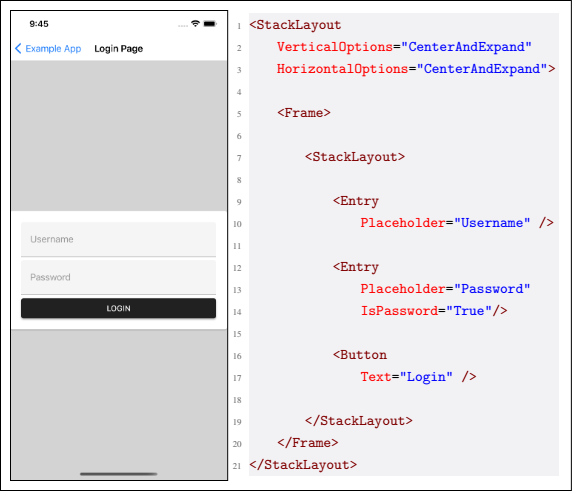
\includegraphics[width=\textwidth,height=\textheight,keepaspectratio]{Images/CrossPlattformFrameworks/ExamplePage.png}
 \caption{Darstellung einer exemplarischen Login-Page}
 \label{fig:ExamplePage}
\end{figure}

Mithilfe der Gegenüberstellungen von \ac{ui}-Elementen und Widgets,  kann anschließend eine Transformation des Xamarin.Forms Layout-Baums zu dem Flutter Widget-Baum durchgeführt werden.  Zur Verdeutlichung wird in Abbildung \ref{fig:LayoutTrees} eine Baumstruktur verwendet,  welche die Verschachtelung innerhalb der Benutzeroberfläche zogt.  Das übergeordnete \glq StackLayout\grq{} von Xamarin.Forms sorgt durch \glq CenterAndExpand\grq{}  als Eigenschaftswert für eine zentrierten Darstellung.  In Flutter übernimmt dies das \glq Center\grq{} Widget.  Für alle  Steuerelemente des obigen Quelltextes wird auf in diesem Kapitel verwiesene Widgets zurückgegriffen. 

\begin{figure}[!ht]
 \includegraphics[width=\textwidth,height=\textheight,keepaspectratio]{Images/CrossPlattformFrameworks/Gegenüberstellung.png}
 \caption{Layout-Baum Überführung von Xamarin.Forms zu Flutter}
 \label{fig:LayoutTrees}
\end{figure}

Um die Funktionsfähigkeit des Widget-Baums sicherzustellen,  wird er innerhalb einer Flutter-App realisiert, siehe Quelltext \ref{lst:LoginPage}, und das visuelle Ergebnis mit der in Abbildung \ref{fig:ExamplePage} dargestellten Xamarin-Forms App verglichen. 

\lstinputlisting[label={lst:LoginPage},caption={Exemplarische LoginPage in Dart} , language=Dart]{SourceCode/FlutterLoginPage.Dart} 

Bei der Ausführung dieser App fällt auf,  dass visuelle Unterschiede im Vergleich zu der vorher entwickelten Xamarin.Forms Variante existieren.  Im oberen linken Teil der Abbildung \ref{fig:LoginPageFlutter} wird das zentrale Element des Login-Formulars dargestellt, wobei im Gegensatz zur Xamarin.Forms Variante die Abstände zwischen den Eingabefeldern fehlen.  Außerdem ist der Login-Button nicht über die verfügbare Breite gestreckt.  Abstände, die das \glq StackLayout\grq{} automatisch zwischen Elemente legt,  müssen in Flutter durch das \glq Padding\grq{} Widget gesondert nachgestellt werden.  Eine weitere Angleichung ist durch das Widget \glq SizedBox\grq{} durchzuführen,  um die Breite des \glq ElevatedButtons\grq{} anzupassen.  Somit kann der zentrale Bereich des Widget-Baums neu generiert werden,  wie er im unteren linken Bereich der Abbildung \ref{fig:LoginPageFlutter} dargestellt ist.  Der angepasste Quelltext,  siehe hierzu auch  \hyperref[chap:OptimizedLoginPage]{Anhang II},  erzeugt durch oben genannte Flutter Anpassungen eine Login-Ansicht mit dem im rechten Teil angezeigten \ac{ui}, die der Xamarin.Forms Variante sehr nahekommt.

\begin{figure}[!ht]
 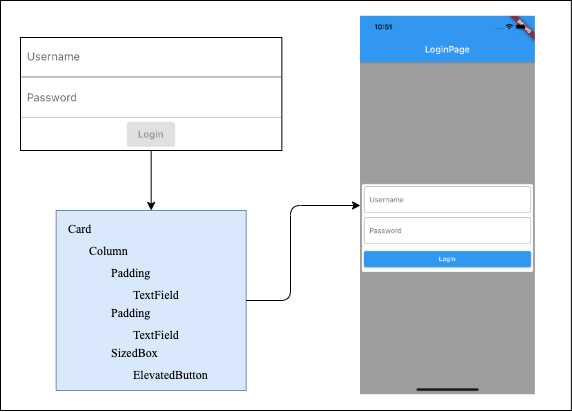
\includegraphics[width=\textwidth,height=\textheight,keepaspectratio]{Images/CrossPlattformFrameworks/FlutterLoginPage.png}
 \caption{Flutter LoginPage Screenshot und Widget-Baum}
 \label{fig:LoginPageFlutter}
\end{figure}

Durch diese Validierung ist ein Beleg für die Annahme,  dass der Austausch von \ac{ui}-Elementen eine App mit vergleichbarer Benutzeroberfläche generieren kann,  erbracht. Jedoch ist für die erfolgreiche Übersetzung von Xamarin.Forms nicht nur die Analyse der Ansichten von elementarer Bedeutung, sondern auch die Berücksichtigung der Eigenschaften und ihrer Kombinationen sowie der nicht im Quelltext ersichtlichen Standardwerte.


